\chapter{Interactive v2 Workload}
\label{sec:interactive-v2}

\subsection*{Related Publications}

A description of the workload (covering reads and inserts) is available in the paper published at TPCTC 2023~\cite{DBLP:journals/corr/abs-2307-04820}.

\begin{itemize}
    \item \textbf{Complex read-only queries.} See \autoref{sec:interactive-complex-reads}.
    \item \textbf{Short read-only queries.} See \autoref{sec:interactive-short-reads}.
    \item \textbf{Insert operations.} See \autoref{sec:insert-operations}.
    \item \textbf{Delete operations.} See \autoref{sec:delete-operations}.
\end{itemize}

\subsection*{Related Software Components}

\begin{itemize}
    \item Datagen (Spark-based): \url{https://github.com/ldbc/ldbc_snb_datagen_spark}
    \item Driver: \url{https://github.com/ldbc/ldbc_snb_interactive_v2_driver}
    \item Reference implementations: \url{https://github.com/ldbc/ldbc_snb_interactive_v2_impls}
\end{itemize}

%%%%%%%%%%%%%%%%%%%%%%%%%%%%%%%%%%%%%%%%%%%%%%%%%%%%%%%%%%%%%%%%%%%%%%%%%%%%%%
%%%%%%%%%%%%%%%%%%%%%%%%%%%%%%%%%%%%%%%%%%%%%%%%%%%%%%%%%%%%%%%%%%%%%%%%%%%%%%
%%%%%%%%%%%%%%%%%%%%%%%%%%%%%%%%%%%%%%%%%%%%%%%%%%%%%%%%%%%%%%%%%%%%%%%%%%%%%%

\section{Overview}

\begin{figure}[htb]
    \centering
    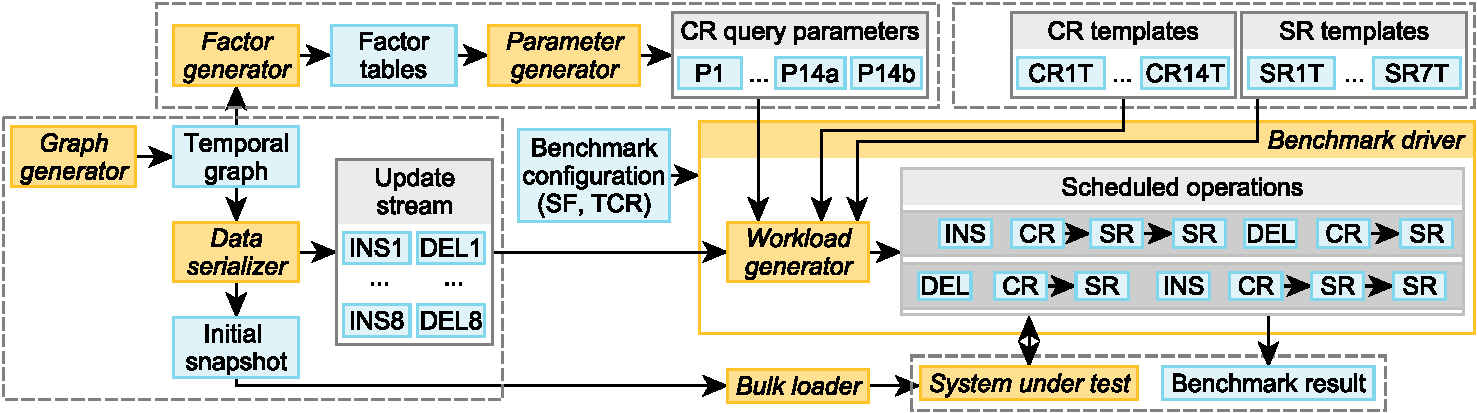
\includegraphics[scale=\yedscale]{figures/interactive-v2-components}
    \caption{
        Components and workflow of the Interactive~v2 workload.
        The corresponding sections are shown in green circles \Circled{\textsf{\scriptsize \S}}.
        Legend:
        \fcolorbox{mydarkyellow}{mylightyellow}{{\scriptsize \textit{\textsf{Software component}}}}
        \fcolorbox{mydarkblue}{mylightblue}{{\scriptsize \textsf{Data artifact\vphantom{p}}}}
    }
    \label{fig:interactive-components}
\end{figure}

\section{Operations}

The complex reads and the short reads are identical to the ones in \interactivevone, except for query 14, which was replaced to cover the \emph{Cheapest path-finding} choke point.

\paragraph{Cheapest path-finding}
While we strived to keep the changes to the queries minimal, we replaced Q14 due to two reasons.
First, we found the original query in \interactivevone to be ill-suited to the workload as it required the enumeration of \emph{all shortest paths} between two \Persons, which can be prohibitively expensive on large scale factors.
% It is in fact intractable according to its theoretical complexity.
%
% A well-constructed adversarial example can result in an exponential number of paths for the number of edges, I think:
%
%   --o--   --o--   --o--   --o--   --o--  
%  /     \ /     \ /     \ /     \ /     \ 
% o---o---o---o---o---o---o---o---o---o---o
%  \     / \     / \     / \     / \     / 
%   --o--   --o--   --o--   --o--   --o--  
%
% This graph has 3^5 paths for just 21 nodes and 30 edges.
%
% Note that while this pattern can occur in the LDBC social graph, its length is usually 4 (especially with the new parameter curation where the path is *guaranteed* to be 4).
% This which means it only produces a quadratic (~d^2) number of paths, which is manageable.
%
% Still, "all shortest paths" is a strange kernel that IMHO isn't very useful and we were right to replace it.  
Second, we introduced a new choke point,
\textsf{CP-7.6}
\emph{Cheapest path-finding,}%
\footnote{
    The term \emph{shortest paths} refers to the problem of finding \emph{unweighted shortest paths}, which can be solved with the BFS algorithm.
    We use \emph{cheapest paths} to refer to the \emph{weighted shortest paths} problem which can be solved using \eg Dijkstra's algorithm.
}
a key computational kernel and a language opportunity for GQL~\cite{DBLP:conf/sigmod/DeutschFGHLLLMM22}.
Therefore, we changed Q14 to use \emph{cheapest paths} instead of \emph{all shortest paths}.

\iftoggle{StandaloneWorkloadSpecification}{
    \input{query-cards/interactive-complex-read-01}
\input{query-cards/interactive-complex-read-02}
\input{query-cards/interactive-complex-read-03}
\input{query-cards/interactive-complex-read-04}
\input{query-cards/interactive-complex-read-05}
\input{query-cards/interactive-complex-read-06}
\input{query-cards/interactive-complex-read-07}
\input{query-cards/interactive-complex-read-08}
\input{query-cards/interactive-complex-read-09}
\input{query-cards/interactive-complex-read-10}
\input{query-cards/interactive-complex-read-11}
\input{query-cards/interactive-complex-read-12}
\input{query-cards/interactive-complex-read-13}
\input{query-cards/interactive-complex-read-14-v2}

}{
    \input{query-cards/interactive-complex-read-14-v2}
}

\iftoggle{StandaloneWorkloadSpecification}{
    \section{Insert Operations}
    \label{sec:insert-operations}
    \input{query-cards/interactive-insert-01}
\input{query-cards/interactive-insert-02}
\input{query-cards/interactive-insert-03}
\input{query-cards/interactive-insert-04}
\input{query-cards/interactive-insert-05}
\input{query-cards/interactive-insert-06}
\input{query-cards/interactive-insert-07}
\input{query-cards/interactive-insert-08}

}

\iftoggle{StandaloneWorkloadSpecification}{
    \section{Delete Operations}
    \label{sec:delete-operations}
    \input{query-cards/delete-01}
\input{query-cards/delete-02}
\input{query-cards/delete-03}
\input{query-cards/delete-04}
\input{query-cards/delete-05}
\input{query-cards/delete-06}
\input{query-cards/delete-07}
\input{query-cards/delete-08}

}

\section{Parameter curation}
\label{sec:parameter-curation}

% \subsection{The need for parameter curation}
% \label{sec:parameter-curation-motivation}

To prevent caching query results, the \snbinteractivevtwo driver instantiates the parameterized complex read (\CR) query templates with different \emph{substitution parameters} (\aka parameter bindings).
% Selecting parameters that lead to stable query runtimes is non-trivial.
% The key reason for this is that the LDBC social network graph exhibits a realistic highly skewed distribution~\cite{DBLP:conf/tpctc/PhamBE12} where some \Person nodes have a large number of outgoing edges while others only have a few connections.
% This has a significant impact on runtimes: if query parameters are selected using uniform random sampling, query runtimes will be unstable, often leading to multimodal distributions which spread across many orders of magnitude~\cite[Figure 4(e)]{DBLP:journals/pvldb/SzarnyasWSSBWZB22}.
However, the na\"ive approach (using a uniform random sampling of parameters and ignoring updates)
leads to unstable runtimes,
which compromise both the benchmark's understandability and reproducibility.
To ensure stable runtimes, LDBC invented \emph{parameter curation} techniques, which select parameters that produce query runtimes with a unimodal (preferably Gaussian) distribution~\cite{DBLP:conf/tpctc/GubichevB14,DBLP:journals/pvldb/SzarnyasWSSBWZB22}.

\subsection{Building blocks for parameter curation}

\paragraph{Temporal bucketing}
\label{sec:temporal-bucketing}
%
To ensure that operations are always executable, \ie they avoid targeting nodes that are yet to be inserted or ones that are already deleted, the parameter curation process in \interactivevtwo employs \emph{temporal bucketing}.
Namely, we create a parameter bucket for \emph{each day in the simulation time of the update streams},
\ie each day in the simulation time has its own distinct set of parameters.
This is a novel feature in \interactivevtwo{} -- previous SNB benchmarks lacked this feature and only selected parameters from the \emph{initial snapshot}.

\paragraph{Factor tables}
As shown in \autoref{fig:interactive-components}, the parameter generation is a two-step process.
The \emph{factor generator} produces \emph{factor tables}, which contain data cube-like summary statistics~\cite{DBLP:journals/datamine/GrayCBLRVPP97} of the temporal graph such as the number of \Messages for friends.
The factor generator is executed in a distributed setup using Spark as this computation includes expensive joins over large tables,
\eg $\knows(\snbperson, \snbfriend) \bowtie \hasCreator(\snbperson, \snbcomment)$.
% this is really a factor as part of the personNumFriendOfFriendComments table

% + temporal information is also required
% \todo{I'm not 100\% sure where this comes from.}

\subsection{Parameter curation for relational queries}

For relational queries (without path-finding), we based our parameter generation on two techniques.

\paragraph{(1) Selecting windows}
%
To select the parameters that are expected to yield similar runtimes, we look for windows with the smallest variance for a given value using SQL window functions.
The parameters are first sorted and grouped together based on their difference in frequency.
Groups that are smaller than a given minimum threshold are discarded to select a group of
parameters large enough to generate a sufficient amount of parameters.
From the latter, we select
the group with the smallest standard deviation.

\paragraph{(2) Selecting distributions}
%
For queries where we want to select parameters that are correlated or anti-correlated, we use factor tables encoding possible combinations (\eg \texttt{countryPairsNumFriends} for \CR[3]):
we select values near a high percentile for the correlated and a low percentile for the anti-correlated case.

\paragraph{Generating the parameters}
%
The parameter candidates discovered by the previous approaches are stored in temporary tables.
The parameter generation step uses these tables to select parameters for each day in the update stream.

% The parameter curation first searches for parts in the factor tables with the smallest variance across for each
% column, called \emph{windows}.
% For each column, the windows are then merged with windows also having the smallest variance.
% This is repeated until there are no windows left or the
% last column is reached.
% The output of the parameter generation is a file for each query containing the substitution parameters.


% This approach significantly increases the complexity of parameter curation as parameter sets 
% makes parameter generation more expensive as the parameter generator needs to generate 33~parameter sets (Nov 29 to Dec 31, 2012).
% This makes the parameter generators performance improvements even more important.

\subsection{Parameter curation for path-finding queries}
\label{sec:path-curation}

\paragraph{The effect of deletes}
%
A key distinguishing feature of graph data management systems is their first-class support for path queries~\cite{DBLP:journals/csur/AnglesABHRV17}.
We demonstrate why ensuring stable query runtimes for path queries is particularly challenging through the example of \autoref{fig:paths}, where we query for the (unweighted) shortest path between \emph{Ada} and \emph{Bob} over a dynamic graph.
Initially, at $t = 1$, the length of the shortest path is 4~hops.
Then, the edge between \emph{Carl} and \emph{Dan} is deleted, making \emph{Ada} and \emph{Bob} unreachable from each other at $t = 2$.
Finally, a new edge is inserted between \emph{Carl} and \emph{Bob}, yielding a shortest path of length 3 at $t = 3$.
This illustrates how a given input parameter (a pair of \Persons) can oscillate between being reachable and being in disjoint connected components over a short period.
To ensure stable query runtimes for path queries in the presence of inserts and deletes, \interactivevtwo introduces a novel \emph{path curation} algorithm, which produces pairs of \Person nodes whose shortest path length from each other is guaranteed to be exactly $k$ hops at any point during a given day.

\paragraph{Graph construction}
%
The parameter curation algorithm builds two variants of the \Person--\knows--\Person subgraph for each day based on the \emph{temporal graph}:
graph $G_1$ has the inserts applied until the beginning of the day and the deletes applied until the end of the day,
while $G_2$ has the deletes applied until the beginning of the day and the inserts applied until the end of the day.
For a given pair of \Person nodes, their shortest path length in $G_1$ is an upper bound $k_\mathrm{upper}$ on their shortest path length at any point in the day -- when the inserts during the day are gradually applied, the shortest path length can only become shorter.
Conversely, $G_2$ gives a lower bound $k_\mathrm{lower}$ for the shortest path -- the deletes can only make the shortest path length become longer.

\paragraph{Parameter selection}
The bounds provided by $G_1$ and $G_2$ guarantee for the shortest path length $k$ that $k_\mathrm{lower} \leq k \leq k_\mathrm{upper}$ will hold at any point during the day.
We can ensure that $k$ will stay constant during the day by selecting \Person pairs where $k_\mathrm{lower} = k_\mathrm{upper}$ holds.
To this end, we select pairs who are exactly 4~hops apart in both $G_1$ and $G_2$, hence they will be always~4 hops apart during the given day.
Unreachable pairs of nodes can be generated by calculating the connected components of $G_2$ and selecting nodes from disjoint components.
The path curation for both the reachable and the unreachable cases is implemented using the NetworKit graph algorithm library~\cite{lit:networkit}.

\newsavebox{\largestimage}
\begin{figure}[htb]
    \vspace{-2.5ex}
    \savebox{\largestimage}{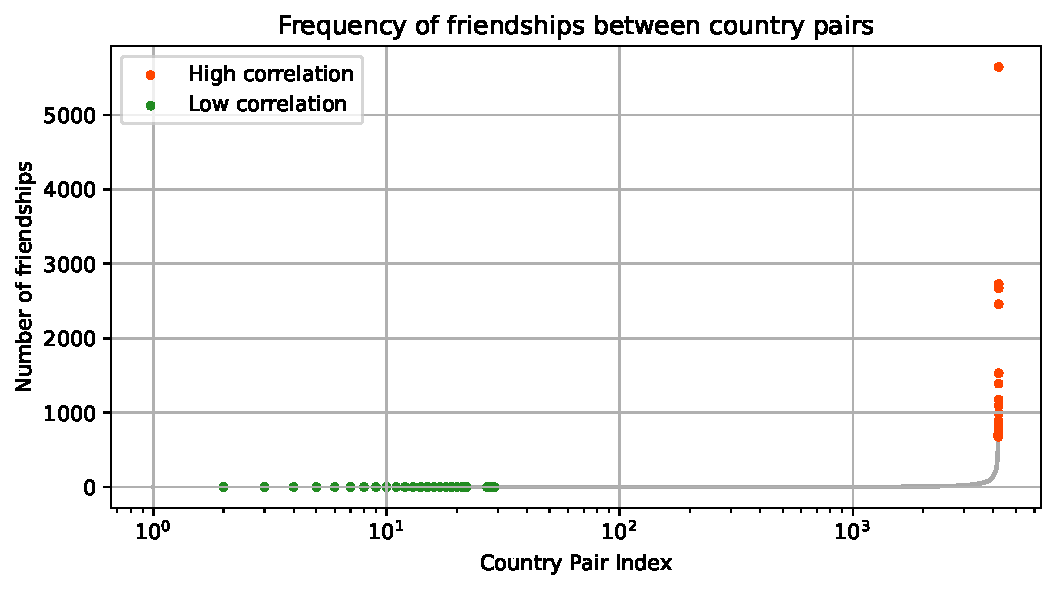
\includegraphics[width=.61\textwidth]{figures/paramgen/paramgen-frequency-disc-countries}}%
    \begin{subfigure}{0.36\textwidth} 
        \centering
        \raisebox{\dimexpr.5\ht\largestimage-.5\height}{%
            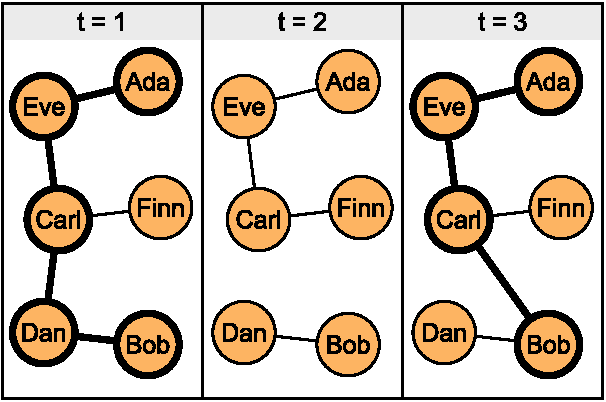
\includegraphics[width=\textwidth]{figures/paths-small}
        }
        \caption{
            Shortest path (denoted with thick lines) between \emph{Ada} and \emph{Bob} in the presence of updates.
        }
        \label{fig:paths}
    \end{subfigure}
    \hspace{2mm}
    \begin{subfigure}{0.61\textwidth}
        \centering
        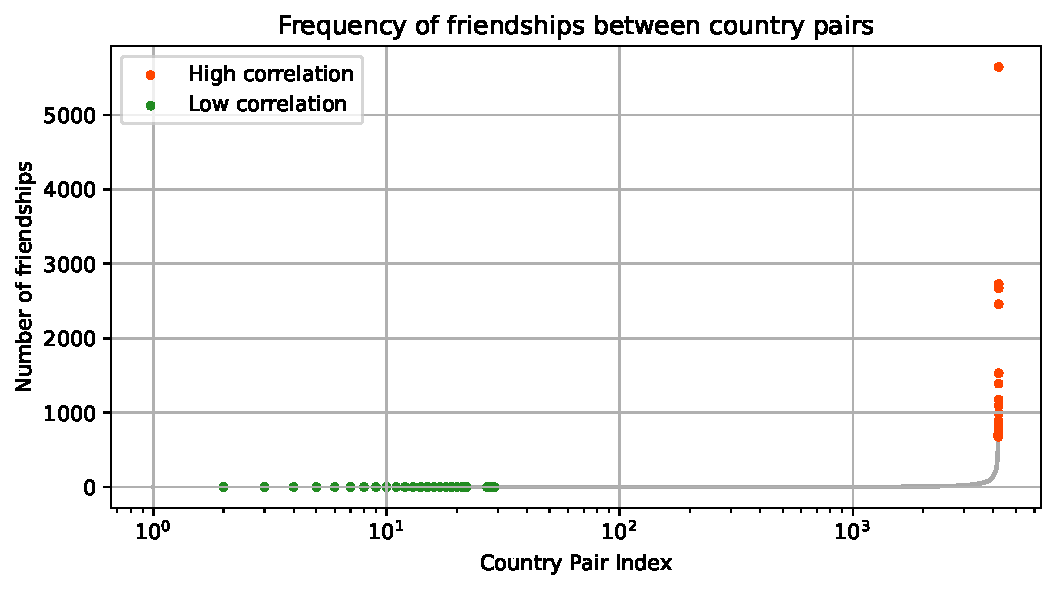
\includegraphics[width=\linewidth]{figures/paramgen/paramgen-frequency-disc-countries}
        \vspace{-3ex}
        \caption{
            Pairs of \Countries in the \texttt{countryPairsNum\-Friends} factor table representing the number of friendships between both \Countries.
            %{percentile\_disc} function. Correlated \Countries (red) are selected using percentile $1.0$ and anti-correlated \Countries (green) are selected using percentile $0.01$.
        }
        \label{fig:paramgen-frequency-disc-countries}
    \end{subfigure}
    \caption{Example graph and distribution for path curation.}
    \label{y}
    \vspace{-4.5ex}
\end{figure}

\subsection{Query variants}
\label{sec:query-variants}

The new workload introduces variants for three queries:
\CR[3], \CR[13], and \CR[14].

\paragraph{\CR[3]: Correlated \vs anti-correlated Countries}
\label{sec:cr3-variants}
%
We introduce variants for \CR[3]:
variant \CR[3(a)] starts from \Countries that have a high correlation in the friendship network,
while
variant \CR[3(b)] starts from \Countries that have a low correlation of friendships between.
To generate these inputs, we use the \texttt{countryPairsNumFriends} factor table visualized in \autoref{fig:paramgen-frequency-disc-countries} and select values at percentile~1.00 for variant~\texttt{(a)} and percentile~0.01 for variant~\texttt{(b)}.

\paragraph{\CR[13] and \CR[14]: Reachable \vs unreachable Persons}
%
Path queries are expected to have different runtimes if there is a path \vs when there is no path.
While the performance characteristics vary highly between systems, in principle, the ``no path'' case should be simpler in the SNB graph, where one of the nodes is always in a small connected component.
To distinguish between these cases, we have two variants for the two path queries \CR[13] and \CR[14].
For variants~\snbOperation{(a)} we select \Person pairs which \emph{do not have a path},
and for variants~\snbOperation{(b)} we select pairs which \emph{have} a path of length~4.
% (guaranteed by path curation, see \autoref{sec:path-curation}).

\subsection{Parameter generator implementation}
\label{sec:paramgen-implementation}

% \paragraph{DuckDB SQL queries}
%
The parameter generator is implemented in Python using NetworKit~\cite{lit:networkit} and SQL queries executed by DuckDB~\cite{DBLP:conf/sigmod/RaasveldtM19}.
% We opted to use DuckDB for multiple reasons:
% it is an embeddable RDBMS with zero setup costs,
% it is optimized for join- and aggregation-heavy analytical queries,
% and it supports the aggregate functions%
% \footnote{\eg \texttt{percentile\_disc()}, see \url{https://duckdb.org/docs/sql/aggregates.html}}
% and window functions%
% \footnote{\eg \texttt{lag()}, see \url{https://duckdb.org/docs/sql/window_functions.html}}
% required by our queries.
%
%\paragraph{Scalability}
%
Based on our experiments in~\cite[Figure~4.3]{david-puroja-msc}, the new parameter generator is scalable.
Even with the significant extra work performed for temporal bucketing,
it outperforms the old parameter generator by more than $100\times$ on SF\numprint{1000},
and finishes in less than 1.5 hours on SF\numprint{10000}.
